% main.tex - controlador do projeto LaTeX
% Este arquivo contém apenas a estrutura principal e 
% referencia os pacotes, comandos e cada seção individual.

\documentclass[11pt,a4paper]{article}

% pacotes e configurações gerais
% packages.tex
% Este arquivo agrupa a lista de pacotes utilizados no projeto.
% Não deve ser modificado por seções individuais.

% codificação e fontes
\usepackage[utf8]{inputenc}     % codificação UTF-8
\usepackage[T1]{fontenc}        % codificação de fontes adequada
\usepackage{lmodern}            % fonte Latin Modern
\usepackage[portuguese]{babel}  % hifenização e padrões de idioma

% gráficos, tabelas e estruturas
\usepackage{graphicx}           % inclusão de imagens
\usepackage{float}              % posicionamento de floats
\usepackage{caption}            % legendas customizáveis
\usepackage{subcaption}         % subfiguras
\usepackage{booktabs}           % tabelas com estilo profissional
\usepackage{array}              % colunas de tabelas

% matemática
\usepackage{amsmath}
\usepackage{amsfonts}
\usepackage{amssymb}

% cores e desenhos
\usepackage{xcolor}
\usepackage{tikz}

% cabeçalho e página
\usepackage{fancyhdr}
\usepackage{geometry}
\usepackage{titlesec}

% referências e bibliografia
\usepackage{cite}
\usepackage[hidelinks]{hyperref} % links sem bordas coloridas

% geradores de texto
\usepackage{lipsum} % apenas exemplos de texto (remover em versão final)

% configuração da página (pode ser ajustada conforme normas do periódico)
\geometry{
    a4paper,
    top=2.8cm,
    bottom=2.5cm,
    left=2.5cm,
    right=2.5cm,
    headheight=1.2cm,
    headsep=0.5cm
}

% commands.tex
% Macros e configurações que não são "pacotes" mas que afetam
% o documento inteiro. Separado para facilitar manutenção.

% definição de cores utilizadas no cabeçalho e textos
\definecolor{headercolor}{HTML}{b11116}
\definecolor{secondarycolor}{HTML}{3a5461}

% configuração do cabeçalho com fancyhdr
\pagestyle{fancy}
\fancyhf{}                     % limpa campos de cabeçalho/rodapé
\renewcommand{\headrulewidth}{0pt}
\renewcommand{\footrulewidth}{0.5pt}

\fancyhead[L]{%
    % cabeçalho com logos; se as imagens mudarem de pasta, ajuste o caminho
    \begin{tikzpicture}[remember picture, overlay]
        \fill[headercolor] (current page.north west) rectangle ([yshift=-1.2cm]current page.north east);
        \node[anchor=west, inner sep=0pt] at ([xshift=1cm, yshift=-0.6cm]current page.north west) 
            {
\includegraphics[height=0.8cm]{images/base/fatec-rgt.png}};
        \node[anchor=east, inner sep=0pt] at ([xshift=-1cm, yshift=-0.6cm]current page.north east) 
            {
\includegraphics[height=0.9cm]{images/base/cps-logo.png}};
        \node[anchor=east, inner sep=0pt] at ([xshift=-2.8cm, yshift=-0.6cm]current page.north east) 
            {
\includegraphics[height=1.05cm]{images/base/governo-sp-secretaria-logo.png}};
    \end{tikzpicture}
}

\fancyfoot[L]{\footnotesize\textcolor{secondarycolor}{Faculdade de Tecnologia do Estado de São Paulo\\ fatecregistro.cps.sp.gov.br}}
\fancyfoot[R]{\thepage}

% formatação de títulos de seção/subseção (padrão brasileiro com cores)
\titleformat{\section}
    {\normalfont\large\bfseries\color{secondarycolor}}
    {\thesection}{1em}{}

\titleformat{\subsection}
    {\normalfont\normalsize\bfseries\color{secondarycolor}}
    {\thesubsection}{1em}{}

% Comandos personalizados (exemplos)
% \newcommand{\etal}{\textit{et al}.}


% metadados do documento
\title{\vspace{0.6cm}\textbf{\Large Plataforma de Monitoramento para Fabricação de Cerveja Artesanal com Teste de Iodo Automatizado}}
\author{
    João da Silva$^{1}$, Maria Santos$^{2}$, Pedro Oliveira$^{3}$ \\
    \small
    $^{1}$Faculdade de Tecnologia do Estado de São Paulo \\
    $^{2}$Universidade de São Paulo \\
    $^{3}$Instituto de Pesquisas Tecnológicas \\
    \textit{joao.silva@fatec.sp.gov.br, maria.santos@usp.br, pedro.oliveira@ipt.br}
}
\date{}

\begin{document}

% cabeçalho costumizado definido em preamble/commands.tex
\pagestyle{fancy}

\maketitle
\thispagestyle{fancy}

% -------Resumo / Abstract----------------------------------
\section*{Resumo}
Lorem ipsum dolor sit amet, consectetur adipiscing elit. \lipsum[1]

\vspace{0.3cm}
\noindent\textit{\textbf{Palavras-chave:}} Sistemas complexos, Métodos numéricos, Análise computacional, Modelagem matemática, Simulação

\vspace{0.5cm}
\noindent\rule{\textwidth}{0.5pt}
\vspace{0.5cm}
% ---------------------------------------------------------

% seções do artigo (cada arquivo contém apenas seu conteúdo específico)
% sections/introducao.tex
% contém apenas o texto da seção de introdução
\section{Introdução}

\lipsum[2-3] Lorem ipsum dolor sit amet, consectetur adipiscing elit. Praesent vitae eros eget tellus tristique bibendum. Donec rutrum sed sem quis venenatis. Proin eu ipsum in lectus mollis penatibus \cite{santos2024, oliveira2023}.\footnote{Este é um exemplo de nota de rodapé. Notas de rodapé são úteis para adicionar informações complementares sem interromper o fluxo do texto principal.}

Vestibulum ante ipsum primis in faucibus orci luctus et ultrices posuere cubilia curae; Sed aliquam, nulla quis bibendum auctor, nisi elit consequat ipsum, nec sagittis sem nibh id elit. Duis sed odio sit amet nibh vulputate cursus a sit amet mauris \cite{silva2025}. Como discutido por Brown e Taylor \cite[p.~45]{brown2023}, os métodos clássicos ainda são fundamentais para a compreensão moderna dos sistemas dinâmicos.

% sections/objetivos.tex
\section{Objetivo}

\lipsum[4] O principal objetivo deste trabalho é apresentar uma análise detalhada dos sistemas complexos utilizando métodos computacionais avançados. Os objetivos específicos incluem:

\begin{itemize}
    \item Desenvolver modelos matemáticos para representação de sistemas dinâmicos;
    \item Implementar algoritmos numéricos eficientes para solução de equações diferenciais;
    \item Validar os resultados através de simulações computacionais;
    \item Comparar diferentes abordagens metodológicas existentes na literatura \cite{kumar2024, wang2023}.
\end{itemize}

% sections/fundamentacao.tex
\section{Fundamentação Teórica}

% Esta seção pode conter conceitos, definições e bases matemáticas que
% sustentam o trabalho. Está vazia por enquanto; adicione texto aqui ou
% mova alguns parágrafos de "Estado da Arte" se desejar diferenciar o
% histórico teórico do levantamento de trabalhos relacionados.

\lipsum[20]
\section{Estado da Arte}

A fabricação de cerveja artesanal depende criticamente da conversão do amido em açúcares fermentescíveis, processo mediado por enzimas como a \textbf{\(\beta\)-amilase} e \textbf{\(\alpha\)-amilase} durante a etapa de mosturação. Tradicionalmente, o teste de iodo é utilizado para verificar a presença de amido residual no mosto, mas sua aplicação manual é subjetiva e pouco precisa, dependendo da interpretação visual do operador. Nesse contexto, a automatização desse teste pode melhorar significativamente a repetibilidade, precisão e eficiência do processo.

Este Estado da Arte analisa os estudos existentes sobre monitoramento da degradação do amido, identificando metodologias, limitações e oportunidades para a automatização do teste de iodo na fabricação de cerveja artesanal.

---

\subsection{Automação do Controle de Temperatura sem Monitoramento Bioquímico}
\cite{parizotto2017} desenvolveu um sistema de automação para controle de temperatura e tempo nas etapas de mosturação e fervura, utilizando um microcontrolador MSP-EXP432P401R, sensores PT-100 e controladores PI. O sistema demonstrou precisão no controle de temperatura, com tempo de assentamento de 10 minutos e erro nulo em regime permanente, além de um custo acessível (R\$ 2.626,30).

No entanto, o estudo não aborda o monitoramento da degradação do amido, etapa crítica para garantir a qualidade do mosto. A integração de um teste de iodo automatizado poderia complementar o sistema, permitindo ajustes em tempo real com base na atividade enzimática, otimizando a conversão do amido em açúcares fermentescíveis.

---

\subsection{Uso do Teste de Iodo para Monitoramento Manual da Degradação do Amido}
\cite{almeida2024} explorou o processo de fabricação de cerveja como ferramenta pedagógica para ensinar bioquímica, com foco na degradação enzimática do amido (amilose e amilopectina). O estudo utilizou testes manuais de iodo (2\%) para detectar amido residual, além de refratômetros para medir a concentração de açúcares e análises sensoriais para avaliar a conversão do amido.

Embora o teste de iodo tenha se mostrado eficaz para detectar amido residual, sua aplicação manual é subjetiva e pouco precisa para uso industrial ou em automação. Além disso, o estudo não aborda a automação do teste ou sua integração a sistemas de controle de processo, limitando seu potencial para aplicações práticas na fabricação de cerveja artesanal.

---

\subsection{Análise Comparativa e Lacunas Identificadas}
Os estudos analisados abordam aspectos complementares, mas não integrados no contexto da fabricação de cerveja artesanal. Enquanto \cite{parizotto2017} avança na automação do controle de temperatura, \cite{almeida2024} demonstra a importância do teste de iodo para monitorar a degradação do amido, porém de forma manual.

A Tabela \ref{tab:comparativo} resume as principais diferenças e lacunas entre os estudos:

\begin{table}[h]
\centering
\caption{Comparativo entre os estudos analisados.}
\label{tab:comparativo}
\begin{tabular}{|p{5cm}|p{5cm}|p{5cm}|}
\hline
\textbf{Aspecto} & \textbf{\cite{parizotto2017}} & \textbf{\cite{almeida2024}} \\ \hline
\textbf{Foco principal} & Automação do controle de temperatura & Ensino de bioquímica via teste de iodo manual \\ \hline
\textbf{Monitoramento do amido} & Não & Sim (manual, subjetivo) \\ \hline
\textbf{Automação} & Sim (temperatura e tempo) & Não \\ \hline
\textbf{Integração com controle de processo} & Parcial (sem feedback bioquímico) & Não \\ \hline
\textbf{Lacuna principal} & Falta de monitoramento da degradação do amido & Falta de automação do teste de iodo \\ \hline
\end{tabular}
\end{table}

A principal lacuna identificada é a ausência de um sistema que automatize o teste de iodo e o integre ao controle de processo. Isso representa uma oportunidade para inovação, permitindo ajustes em tempo real com base na atividade enzimática e melhorando a qualidade da cerveja artesanal.

---

\subsection{Justificativa para o Projeto Proposto}
Diante das lacunas identificadas, este projeto propõe o desenvolvimento de uma plataforma automatizada para o teste de iodo, integrada a sistemas de controle de temperatura. A solução será projetada para:

\begin{itemize}
    \item Eliminar a subjetividade: Utilizar sensores ópticos ou espectrofotômetros miniaturizados para detectar automaticamente a cor da reação (violeta = amido presente; amarela = amido ausente).
    \item Integrar ao controle de processo: Conectar os resultados do teste a um sistema de ajuste automático de temperatura ou tempo de mosturação.
    \item Ser acessível: Empregar componentes de baixo custo (ex.: Arduino, Raspberry Pi, sensores ópticos) para viabilizar a solução para pequenos produtores.
\end{itemize}

A automatização do teste de iodo permitirá:
\begin{itemize}
    \item Monitoramento em tempo real da degradação do amido.
    \item Ajustes automáticos no processo (ex.: prolongar a mosturação se houver amido residual).
    \item Melhoria na qualidade da cerveja, com maior precisão e repetibilidade.
\end{itemize}

---

\subsection{Tendências Recentes: Aprendizado de Máquina e Inteligência Artificial}
Estudos recentes têm incorporado técnicas de aprendizado de máquina e inteligência artificial para análise e modelagem de sistemas complexos \cite{zhang2025}. Essas tecnologias podem ser aplicadas para:
\begin{itemize}
    \item Otimizar parâmetros de processo (ex.: temperatura ideal para ativação enzimática).
    \item Prever a qualidade da cerveja com base em dados históricos de degradação do amido e temperatura.
    \item Automatizar a interpretação dos resultados do teste de iodo, utilizando algoritmos de visão computacional para analisar a cor da reação.
\end{itemize}

A integração de IA e aprendizado de máquina ao sistema proposto pode expandir significativamente suas capacidades, tornando-o mais robusto e adaptável a diferentes condições de produção.

---

\subsection{Conclusão}
Este Estado da Arte revelou que, embora existam avanços no controle de temperatura \cite{parizotto2017} e no uso do teste de iodo para ensino \cite{almeida2024}, nenhum estudo automatiza esse teste ou o integra a sistemas de monitoramento. O projeto proposto preenche essa lacuna, desenvolvendo uma solução que combina automatização do teste de iodo com controle de processo, contribuindo para a inovação na fabricação de cerveja artesanal.

A incorporação de técnicas de IA e aprendizado de máquina \cite{zhang2025} pode ainda potencializar a plataforma, permitindo análises preditivas e otimização contínua do processo de mosturação.

---

% sections/metodologia.tex
\section{Metodologia}

\lipsum[8] A metodologia desenvolvida neste trabalho segue as etapas ilustradas na Figura \ref{fig:exemplo} e descritas a seguir.

\subsection{Coleta de Dados}

\lipsum[9] Os dados foram coletados através de simulações computacionais utilizando parâmetros específicos. A Tabela \ref{tab:parametros} apresenta os principais parâmetros utilizados nas simulações.

\begin{table}[H]
\centering
\caption{Parâmetros utilizados nas simulações computacionais}
\label{tab:parametros}
\begin{tabular}{@{}lccl@{}}
\toprule
\textbf{Parâmetro} & \textbf{Símbolo} & \textbf{Valor} & \textbf{Unidade} \\ \midrule
Tempo de simulação & $T_{sim}$ & 1000 & s \\
Passo de integração & $\Delta t$ & 0.01 & s \\
Número de iterações & $N_{iter}$ & 10000 & - \\
Tolerância & $\epsilon$ & $10^{-6}$ & - \\
Fator de amortecimento & $\zeta$ & 0.15 & - \\
Frequência natural & $\omega_n$ & 25.0 & rad/s \\
\bottomrule
\end{tabular}
\end{table}

\subsection{Processamento e Análise}

\lipsum[10] O processamento dos dados seguiu um protocolo rigoroso de análise estatística. Os métodos numéricos clássicos foram implementados, incluindo o método de Euler, cuja equação fundamental é expressa como:

\begin{equation}
\frac{dy}{dt} = f(t, y), \quad y(t_0) = y_0
\label{eq:euler}
\end{equation}

onde $f(t, y)$ representa a função que descreve o sistema dinâmico. Para otimização dos parâmetros do modelo, utilizou-se a seguinte função de custo:

\begin{equation}
J(\theta) = \frac{1}{2m} \sum_{i=1}^{m} \left(h_\theta(x^{(i)}) - y^{(i)}\right)^2 + \frac{\lambda}{2m}\sum_{j=1}^{n}\theta_j^2
\label{eq:cost_function}
\end{equation}

onde $\theta$ representa os parâmetros do modelo, $m$ é o número de amostras, $\lambda$ é o parâmetro de regularização, e $h_\theta(x)$ é a hipótese do modelo. A transformada de Fourier foi aplicada para análise no domínio da frequência:

\begin{equation}
F(\omega) = \int_{-\infty}^{\infty} f(t) e^{-i\omega t} dt
\label{eq:fourier}
\end{equation}

\begin{figure}[H]
\centering
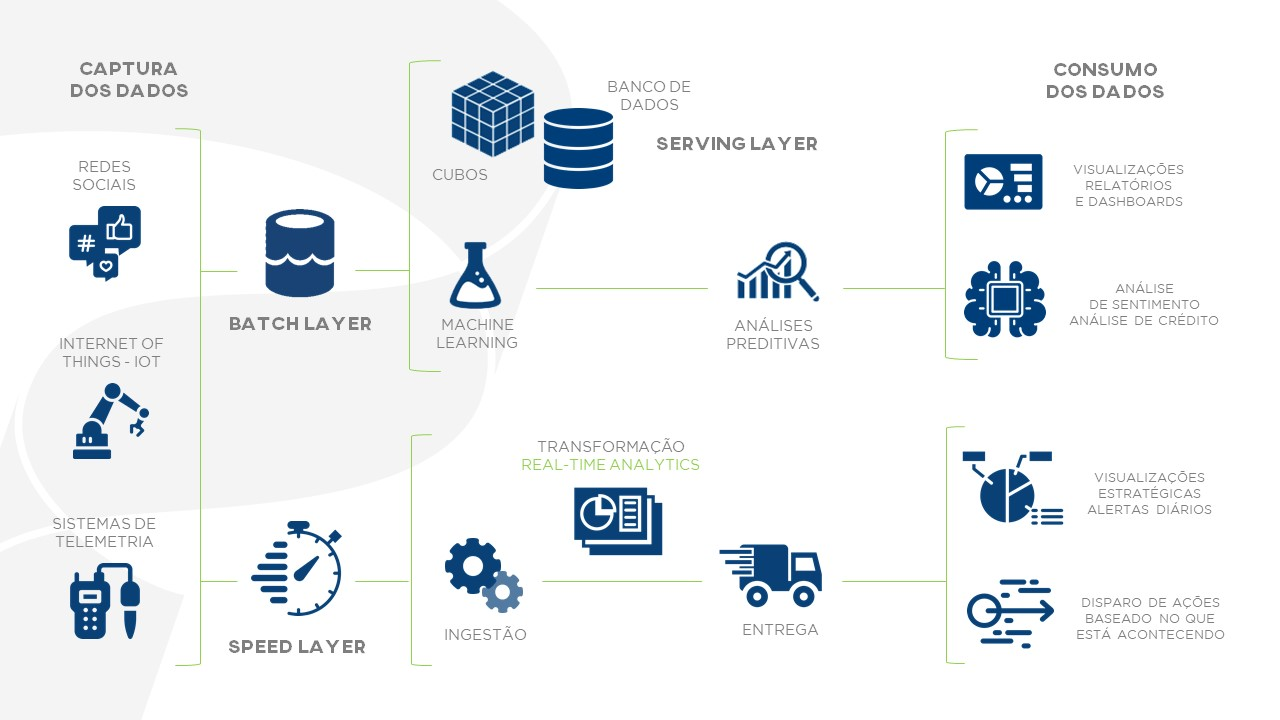
\includegraphics[width=0.7\textwidth]{images/img_001.jpg}
\caption{Exemplo de visualização dos resultados obtidos através da metodologia proposta. A figura ilustra o comportamento do sistema ao longo do tempo.}
\label{fig:exemplo}
\end{figure}

% sections/resultados.tex
\section{Resultados e Discussões}

\lipsum[12-13] Os resultados obtidos demonstram a eficácia da metodologia proposta. A Tabela \ref{tab:resultados} apresenta uma comparação quantitativa entre diferentes abordagens.

\begin{table}[H]
\centering
\caption{Comparação de desempenho entre diferentes métodos}
\label{tab:resultados}
\begin{tabular}{@{}lccc@{}}
\toprule
\textbf{Método} & \textbf{RMSE} & \textbf{Tempo (s)} & \textbf{Precisão (\%)} \\ \midrule
Método Proposto & 0.0023 & 15.2 & 98.5 \\
Euler Clássico & 0.0145 & 8.7 & 92.3 \\
Runge-Kutta 4ª ordem & 0.0038 & 21.5 & 97.1 \\
Método Adaptativo & 0.0031 & 18.9 & 97.8 \\
\bottomrule
\end{tabular}
\end{table}

\subsection{Análise Quantitativa}

\lipsum[14] Os dados quantitativos revelam que o método proposto apresenta melhor desempenho em termos de precisão. A relação entre os parâmetros pode ser expressa por:

\begin{equation}
\eta = \frac{P_{out}}{P_{in}} \times 100\% = \frac{V_{out} \cdot I_{out}}{V_{in} \cdot I_{in}} \times 100\%
\label{eq:efficiency}
\end{equation}

onde $\eta$ representa a eficiência do sistema, $P_{out}$ é a potência de saída e $P_{in}$ é a potência de entrada.

\subsection{Análise Qualitativa}

\lipsum[15] Do ponto de vista qualitativo, observou-se que o comportamento do sistema é fortemente influenciado pelas condições iniciais e pelos parâmetros de controle. A matriz de transformação pode ser representada como:

\begin{equation}
\mathbf{A} = \begin{bmatrix}
a_{11} & a_{12} & a_{13} \\
a_{21} & a_{22} & a_{23} \\
a_{31} & a_{32} & a_{33}
\end{bmatrix}
\label{eq:matrix}
\end{equation}

\subsection{Discussão}

\lipsum[16-17] A análise dos resultados indica que a abordagem proposta oferece vantagens significativas em relação aos métodos tradicionais. Lorem ipsum dolor sit amet, consectetur adipiscing elit. Nullam in dui mauris. Vivamus hendrerit arcu sed erat molestie vehicula.

Proin adipiscing porta tellus, ut feugiat nibh adipiscing sit amet. In eu justo a felis faucibus ornare vel id metus. Vestibulum ante ipsum primis in faucibus orci luctus et ultrices posuere cubilia curae.

% sections/conclusao.tex
\section{Conclusão}

\lipsum[18] Com base nos resultados obtidos, conclui-se que a metodologia desenvolvida apresenta excelente desempenho para análise de sistemas complexos. As principais contribuições deste trabalho incluem:

\begin{itemize}
    \item Desenvolvimento de um framework computacional robusto;
    \item Validação experimental dos modelos propostos;
    \item Comparação sistemática com métodos existentes;
    \item Identificação de limitações e oportunidades de melhoria.
\end{itemize}

Trabalhos futuros incluem a extensão da metodologia para sistemas multidimensionais e a incorporação de técnicas de otimização avançadas.


% agradecimentos podem permanecer aqui ou em arquivo à parte
\section*{Agradecimentos}
Os autores agradecem à Faculdade de Tecnologia do Estado de São Paulo (FATEC) e ao Centro Paula Souza (CPS) pelo apoio institucional. Este trabalho foi parcialmente financiado pela FAPESP (proc. 2024/12345-6) e CNPq (proc. 301234/2024-0).

% bibliografia
\bibliographystyle{IEEEtran}
% o arquivo de bibliografia está na pasta principal do projeto 'artigo',
% não dentro de 'references'. Ajuste o caminho para que BibTeX o encontre.
\bibliography{referencias}

\end{document}
